\documentclass[12pt]{article}

\usepackage[spanish]{babel}
\usepackage[utf8]{inputenc}
\usepackage{graphicx}
\usepackage{geometry}
\usepackage{xcolor}
\usepackage{fancyhdr}
\usepackage{lastpage}
\usepackage{pdfpages}
\usepackage{listings}

\geometry{top=25mm,left=15mm,right=15mm,a4paper}

\pagestyle{fancy}
\fancyhf{}
\lhead{Lenguajes de Programación}
\cfoot{Página \thepage\ de \pageref{LastPage}}

\graphicspath{./}

\begin{document}
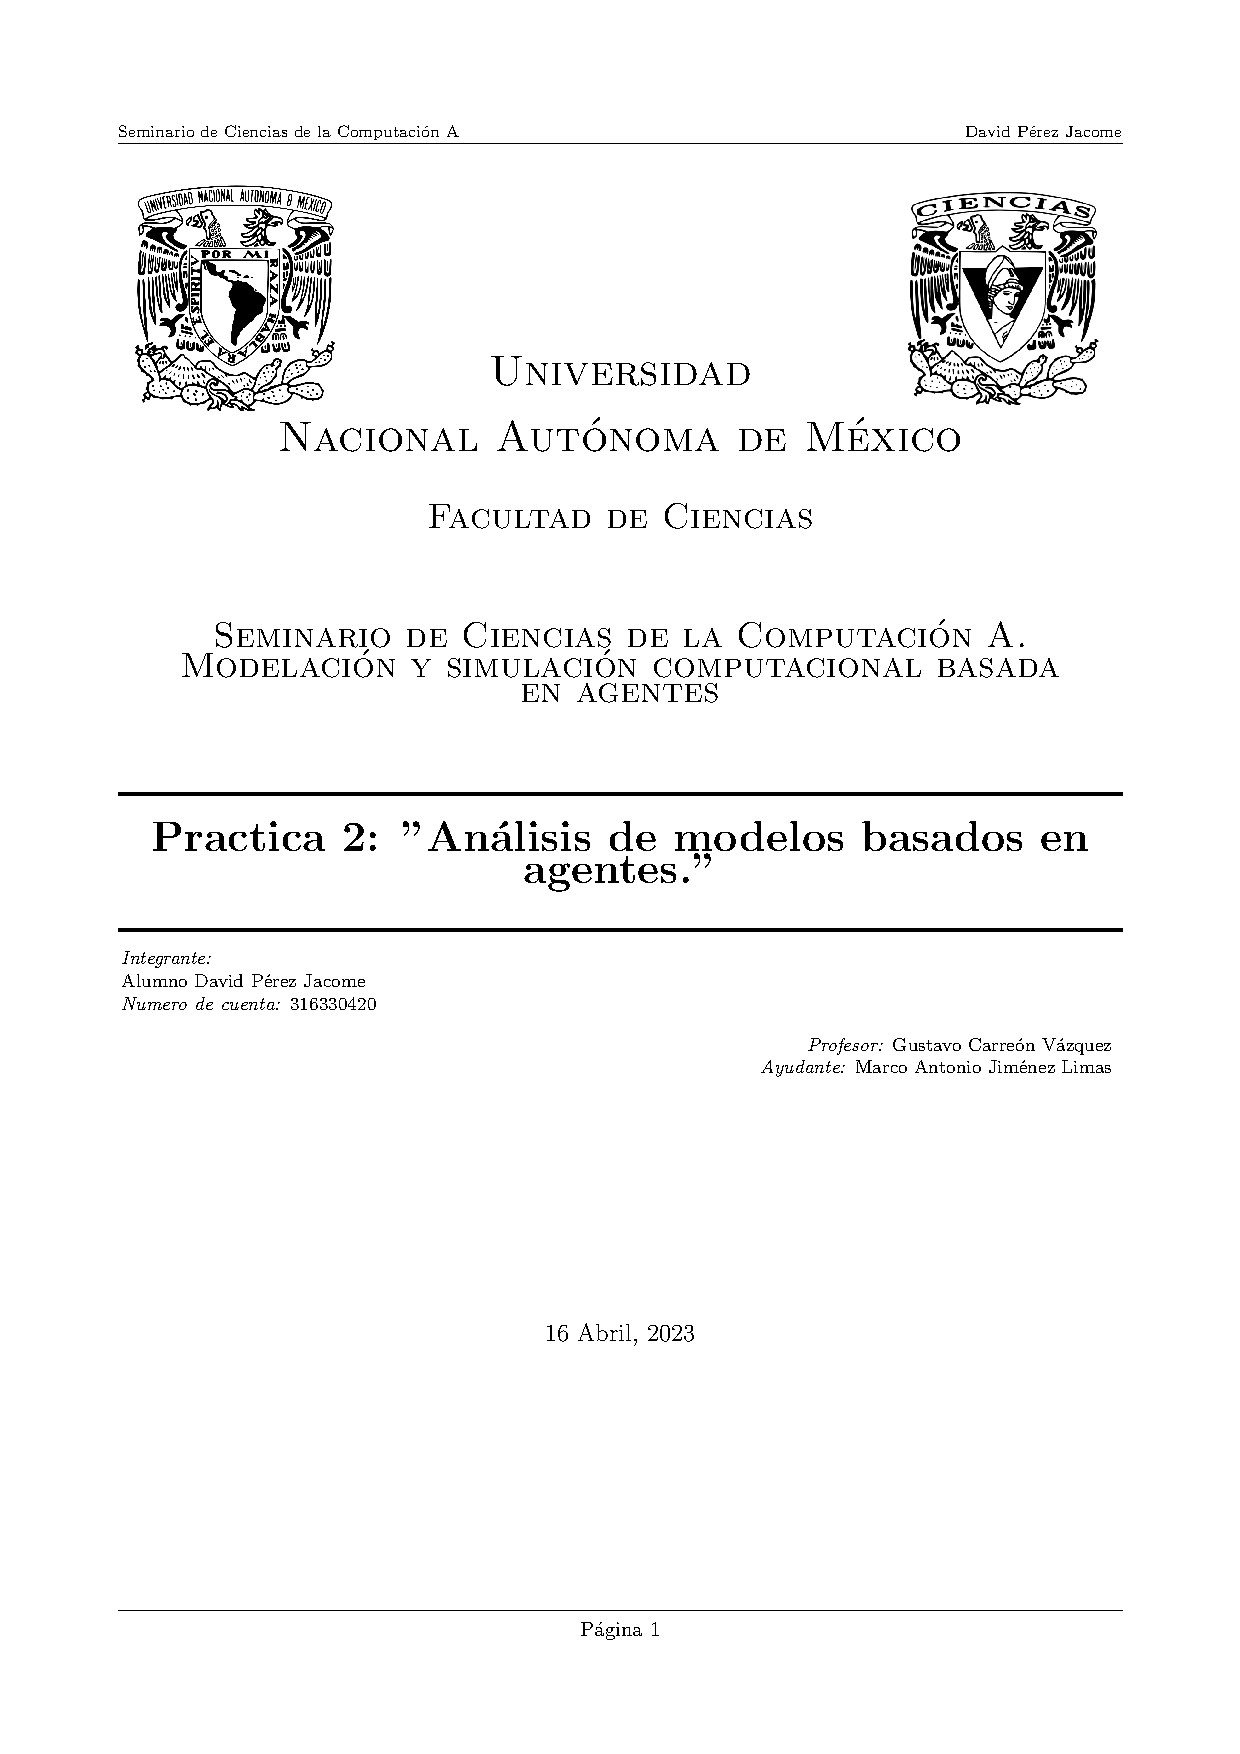
\includepdf{Portada.pdf}
{\color{red} \section*{Practica 2: Análisis de modelos basados en agentes.}}

{\color{blue} \subsection*{Parte 1. Modelo de segregación de Schelling.}}
\vspace{1em}

El modelo propuesto originalmente por Thomas Schelling consiste en dos grupos de agentes, por ejemplo rojos y verdes, que localmente tratan de satisfacer la necesidad de estar con los
de su mismo grupo. De manera general este comportamiento es establecido por un parámetro conocido como porcentaje de \textbf{similitud-requerida} o nivel de tolerancia.\\

Los agentes toman una desición apartir de la información que tienen en su vecindad. Si el agente satisface las condiciones del entorno entonces se queda en su posición actual, de lo contrario
se mueve a otra posición vacia. Esta dinamica local genera como resultado la formación de cúmmulos de agentes del mismo tipo, hay segregación.\\

\textbf{Definición del Sistema:} El sistema se compone de una reticula de $n$ x $n$ donde $n$ se establece entre $50$ y $100$.
Cada celda con posición $(i,j)$ alberga a un agente rojo o verde. El sistema tiene un parámetro de \textbf{densidad poblacional} usualmente se establece en $90\%$ (es decir, $10\%$ de las celdas quedan vacias).
La mitad de la población es color rojo y la otra mitad, color verde. Cada agente toma una celda aleatoriamente.\\

\textbf{Dinámica:} Cada agente en la posición $(i,j)$ se "muda" a un lugar vacio si su vecindad de Moore no cumple con el porcentaje de similitud requerida.\\

{\color{blue} \subsubsection*{Ejercicios:}}

\begin{enumerate}
    \item \textbf{Implmente el modelo} de segregación de Schelling original, pueden usar de base el codigo visto en clase.
    \item 
\end{enumerate}

{\color{blue} \subsection*{Parte 2. Automata Celular Elemental (ACE)}}
\vspace{1em}

Desarrollar un autómata celular con el lenguaje de programación de su elección o usar el codigo base de NetLogo. Implmentar las caracteristicas: (especificaciones pdf original)\\

\begin{enumerate}
    \item Función de transición
    \item Fronteras
    \item Tamaño
    \item Condiciones iniciales
    \item Salida gráfica
\end{enumerate}
{\color{blue} \subsubsection*{Ejercicios:}}

\begin{enumerate}
    \item \textbf{Exploración:} Ejecute algunas de las $256$ reglas del autómata celular a partir de la implementación de su programa con condiciones de frontera periodicas, minimo 100 tiempos de
    evolución y condiciones iniciales aleatorias, Identifique el tipo de dinamica que presenta y a que case pertenece según las cuatro categorías de la Clasificación de Wolfram. Muestre 1 representante de cada clase y adjunte la 
    captura de pantalla.\\
    \textbf{\color{red} RESPUESTA:}\\
    Después de una serie de ejecuciones del programa que implemente en NetLogo para ACE, pude deducir con base a lo visto en clase 4 ejecuciones cada una correspondiente a una clase de las 4 de Wolfram.
    \begin{enumerate}
        \item CLASE I:\\ Regla $255$
        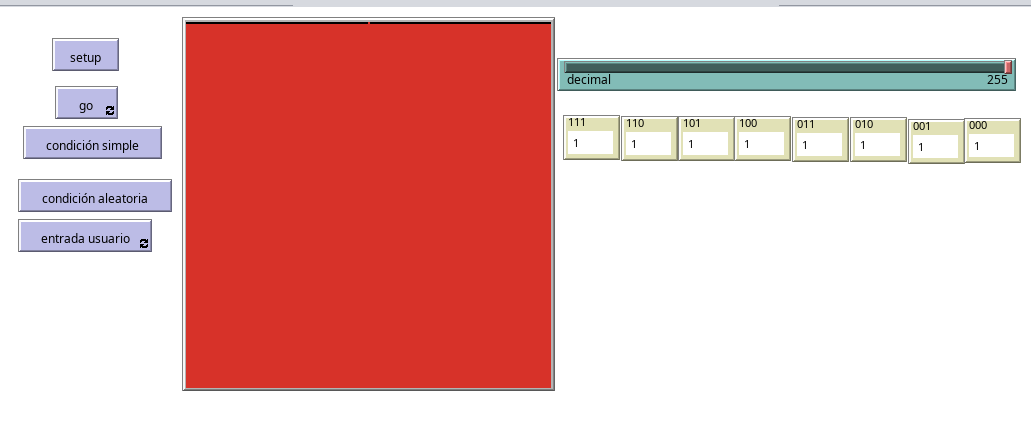
\includegraphics[scale = 0.40]{images/clase1_255.png}
        \item CLASE II:\\ Regla $250$
        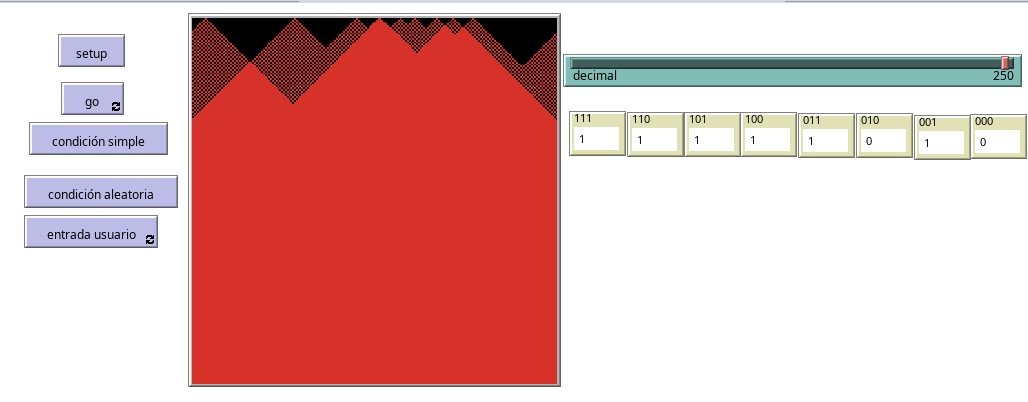
\includegraphics[scale = 0.40]{images/clase2_250.png}
        \item CLASE III:\\ Regla $22$
        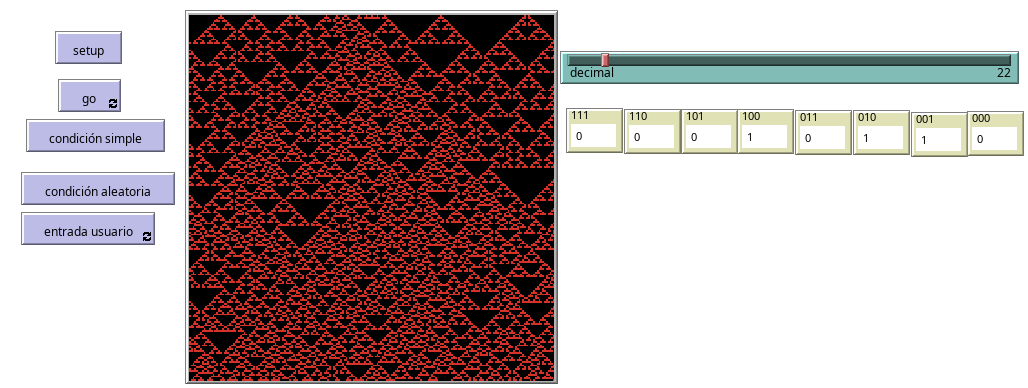
\includegraphics[scale = 0.40]{images/clase3_22.png}
        \item CLASE IV:\\ Regla $54$
        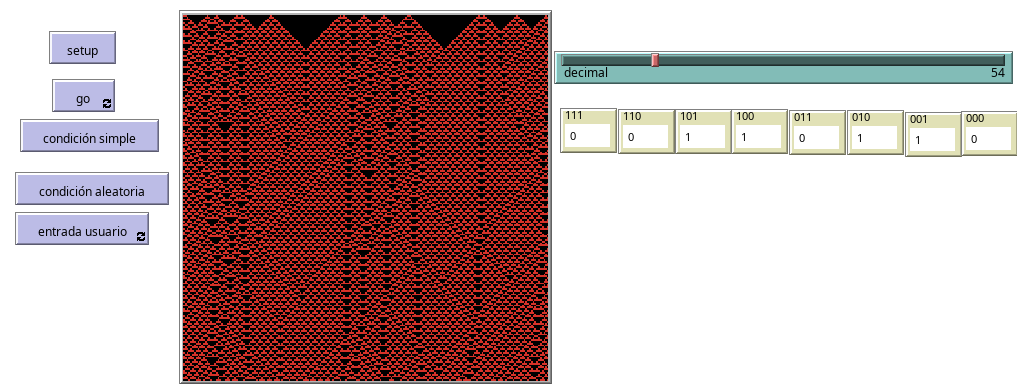
\includegraphics[scale = 0.40]{images/clase4_54.png}
    \end{enumerate} 
    \item Después de explorar todas o algunas de las 256 reglas. ¿Cuál crees que sea la clase más frecuente?\\
    \textbf{\color{red} RESPUESTA:}\\
    A mi parecer y con base a lo visto en clase y lo ejecutado, puedo concluir que pude apreciar una mayor parte de ACE relacionados con la \textbf{Clase II} e incuso en clase vimos que tiene un aproximado de $194$ reglas asociadas, aproximado porque puede que algunas
    esten en la frontera de I  y III.
    \item \textbf{Sensibilidad a condiciones iniciales.} Encuentra un autómata de clase III, perturbe la condición inicial aleatoria por un bit, evolucione y vea las diferencias. ¿La sensibilidad a las condiciones iniciales es una propiedad suficiente para 
    catalogar la dinámica como caotica? (Adjunte imagenes del ACE perturbado, sin perturbar).\\
    \textbf{\color{red} RESPUESTA:}\\
    Para esta parte vamos a ejecutar la regla 90 de Clase III en la \textbf{Fig.1} con una condición inicial simple (patch de en medio) y continuamnete en la \textbf{Fig.2} con un patch más encendido.\\

    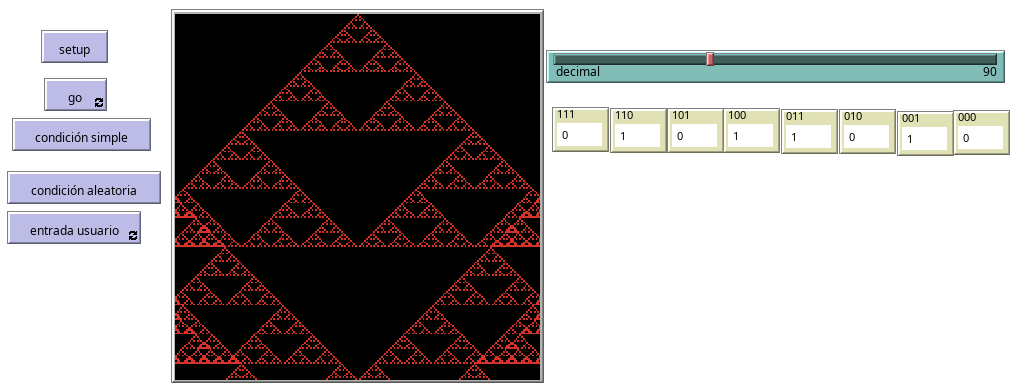
\includegraphics[scale = 0.40]{images/fig1_90.png} FIG.1

    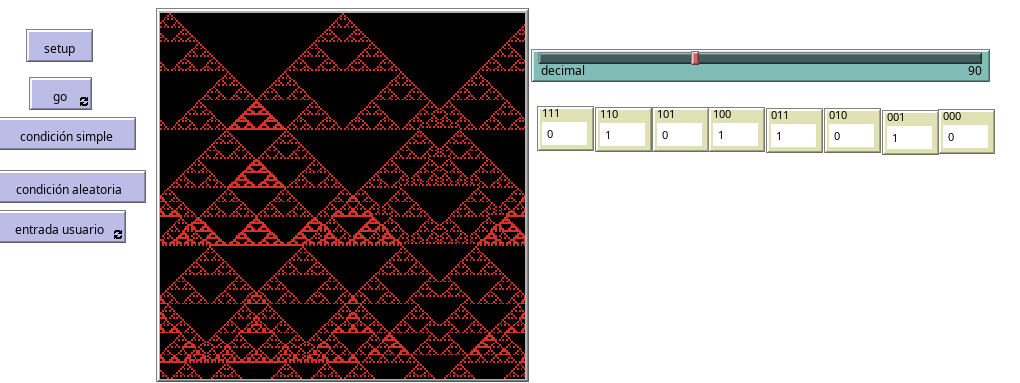
\includegraphics[scale = 0.40]{images/fig2_90.png} FIG.2

    Podemos observar que no es necesaria una perturbación para considerar que es una dinamica caotica, ya que la estructura sigue persistiendo
    y no es tan notorio el cambio.

    \item ¿Qué poder de cómputo tiene la regla 132? y ¿Qué propiedades tiene la regla 30?  Explique y adjunte capturas.\\
    \textbf{\color{red} RESPUESTA:}\\ 
    La regla 132 además de su comportamiento caótico y complejo, su poder de cómputo es limitado debido a la simplicidad de los autómatas celulares elementales en general.

    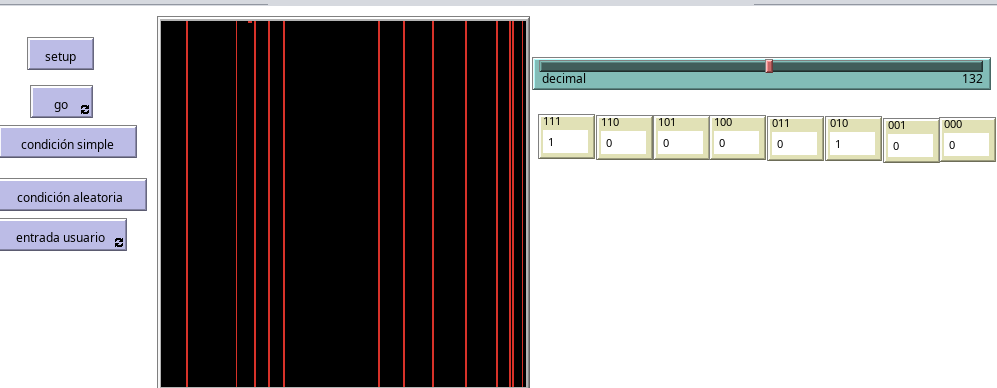
\includegraphics[scale = 0.40]{images/regla132.png}.

    La regla 30 es un ejemplo de un sistema dinámico complejo, lo que significa que exhibe patrones no triviales que emergen de interacciones simples entre sus componentes. Esta complejidad puede manifestarse en patrones simétricos, periódicos o caóticos, que pueden ser
    visualizados a través de las iteraciones de la regla, además comportamiento caótico, lo que significa que incluso pequeñas variaciones en las condiciones iniciales pueden producir resultados muy diferentes a largo plazo.

    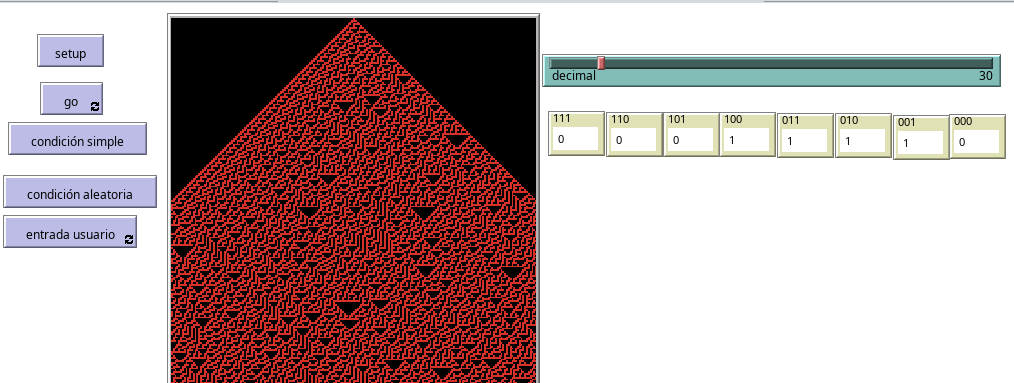
\includegraphics[scale = 0.40]{images/regla30.png}

    \item En las imagenes del documento de la practica se muestra la evolución de la regla 22 con condición inicial simple (una celda negra en el centro) y
    condición inicial aleatoria. Explique lo que sucede con la dinámica.\\
    \textbf{\color{red} RESPUESTA:}\\
    En relacion con ambas figuras podemos concluir que es caotica ya que una variación nos da un automata un tanto más complejo, claro que se puede apreciar su naturaleza, por asi decirlo si nos referimos a as estructuras que se forman,
    pero tambien podemos ver que la entrada al ser aleatoria y tener mas de 2 patch encendidos al ser ejecutado llega a verse cada vez más y más compleja nuestra estructura.

    \item Si el autómata estuviera definido en el alfabeto de 3 estados, ¿Cuántas posibles reglas hay?\\
    \textbf{\color{red} RESPUESTA:}\\
    Si consideramos un autómata celular de una solo dimensión con un alfabeto de 3 estados, cada celda puede tener uno de tres estados diferentes: 0, 1 o 2.
    Si consideramos únicamente los primeros vecinos (las celdas adyacentes a la izquierda y a la derecha), entonces cada celda tiene $3^2 = 9$ posibles combinaciones de estados que podemos utilizar para definir una regla.

Para determinar el número total de reglas posibles, necesitamos determinar cuántas combinaciones de 9 elementos podemos formar con un alfabeto de 3 estados. Esto se puede calcular utilizando la fórmula para combinaciones con repetición, que es:

$C(n + k - 1, k) = C(9 + 3 - 1, 3) = C(11, 3) = 165$

Por lo tanto, hay un total de 165 posibles reglas. 
\end{enumerate}

{\color{blue} \subsection*{Parte 3. Automata Celular Bidimensional "LIFE" }}
\vspace{1em}

El juego de la vida (LIFE), propuesto John Horton Conway, es uno de los
ejemplos más representativos de un autómata celular bidimensional. Su
conjunto de reglas genera una gran cantidad de patrones, que aún hoy en día,
se siguen encontrando.\\

Implemente LIFE usando el codigo visto en clase con las siguientes reglas de actualización, considerando una vecindad de Moore.\\

Para una celda que esta "viva"
\begin{enumerate}
    \item Si tiene uno o cero vecinos "muere" (por soledad).
    \item Si tiene cuatro o más vecinos "muere" (por sobrepoblación).
    \item Si tiene dos o más vecinos "sobrevive".
\end{enumerate}

Para una celda que esta "vacia" o "muerta".
\begin{enumerate}
    \item Si tiene tres vecinos la celda "vive".
\end{enumerate}

El minimo del tamaño de la reticula debe ser de $100x100$.\\

{\color{blue} \subsubsection*{Ejercicios:}}

\begin{enumerate}
    \item En NetLogo coonstruya una gráfica de conteo de celdas vivas a través del tiempo. Ejecute varias veces su programa con una reticula de $100x100$ celdas 
    y condición aleatoria con $50\%$ de celdas ocupadas, ¿en cuánto
    tiempo (ticks) se "estabilizó" la dinámica?, ¿para cualquier configuración
    inicial aleatoria pasará lo mismo? Explique y adjunte una captura de
    pantalla del “view” de agentes y la gráfica de conteo.\\
    \textbf{\color{red} RESPUESTA:}\\
    Al ejecutar el juego de la vida un total de 10 veces, en un promedio obtuve que emepzo en un tiempo de regulación de $231.4$\\

    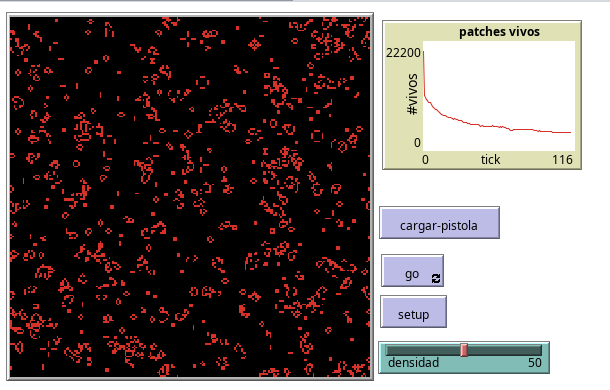
\includegraphics[scale = 0.40]{images/50juego.png}
    
    \item Realice el mismo experimento aumentando la densidad de la condición
    aleatoria a 85\%, ¿sucede lo mismo? Explique.\\
    \textbf{\color{red} RESPUESTA:}\\
    En este caso e sistema se nivela o acaba de una manera más rapida, el ejecutar de igual forma un total de 10 ejecuciones, pude llegar a un promedio de $11.16$
    en el que en tan pocos ticks acaba.\\

    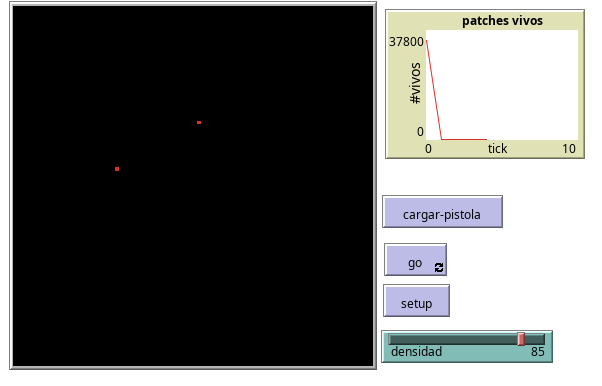
\includegraphics[scale = 0.40]{images/juego85.png}
    
    \item Implemente la "pistola de planeadores" o "Gosper's gun" dada la condición inicial del pdf original.
    Explique la dinamica que se genera, ¿es periódica? ¿qué implicaciones tiene controlar de alguna manera ciertas estructuras en función del tiempo?\\
    \textbf{\color{red} RESPUESTA:}\\
    Sí, la "Gosper's gun" es un patrón periódico en el juego de la vida. Tiene un período de 30 ciclos de reloj, lo que significa que después de 30 iteraciones del juego de la vida, el patrón se repite a sí mismo en su forma original.
    Durante cada período, la "Gosper's gun" dispara una serie de naves espaciales que se mueven hacia afuera y luego desaparecen. Estos movimientos son determinados por las reglas del juego de la vida y por la forma específica en que se organizan las células dentro del patrón.
    El período de la "Gosper's gun" es una de las características que la hacen interesante desde el punto de vista matemático y computacional, ya que permite predecir y simular su comportamiento de manera precisa y eficiente.\\
    El control de estructuras como la "Gosper's gun" podría permitir la creación de patrones de células específicos que pueden usarse para resolver problemas complejos de manera más eficiente. Por ejemplo, se ha demostrado que ciertos patrones de células en el juego de la vida pueden usarse para computación universal, lo que significa que pueden simular cualquier proceso computacional.
    En la biología y la medicina, el control de estructuras en función del tiempo puede permitir la modulación de procesos celulares y fisiológicos, lo que podría tener aplicaciones en el tratamiento de enfermedades y la regeneración de tejidos.
    En la ingeniería y la informática, el control de estructuras en función del tiempo puede permitir la optimización de procesos y sistemas complejos, lo que podría tener aplicaciones en el diseño de algoritmos y sistemas de control.\\

    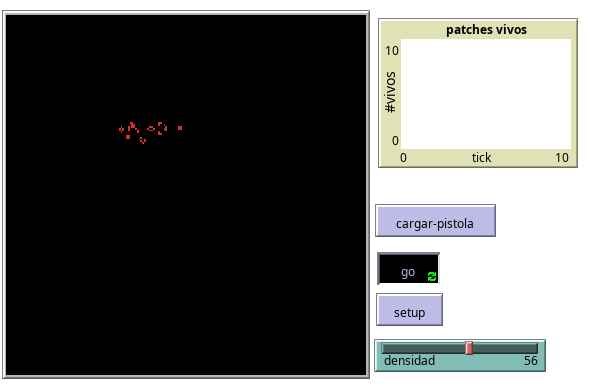
\includegraphics[scale = 0.40]{images/pistola.png}


    \item ¿El juego de la vida es reversible? Explique.\\
    \textbf{\color{red} RESPUESTA:}\\
    No, en general el juego de la vida no es reversible, lo que significa que no se puede determinar el estado anterior del juego a partir del estado actual. Esto se debe a que el juego de la vida no conserva la información necesaria para reconstruir el estado anterior del juego.
    En particular, la evolución del juego de la vida es determinista, lo que significa que el estado actual del juego se determina completamente a partir del estado anterior. Sin embargo, esta evolución no es invertible, ya que hay muchos estados anteriores posibles que pueden llevar al mismo estado actual, lo que se conoce como la propiedad de la no unicidad de la inversión.
    Hay algunas excepciones a esta regla general. Por ejemplo, se ha demostrado que ciertos patrones especiales en el juego de la vida, como los patrones estables y los osciladores, son reversibles. En estos casos, se puede determinar el estado anterior del juego a partir del estado actual, ya que se conserva información suficiente sobre la evolución del patrón.
\end{enumerate}



\end{document}